%!TEX program = xelatex
\documentclass{article}
\usepackage{LaTeX-Submodule/template}

% Additional packages and macros
\usepackage{changepage} % Modify page width
\usepackage{multicol} % Use multiple columns
\usepackage{titlesec} % Modify section heading styles

\geometry{
	a4paper,
	margin = 10mm
}

\pagenumbering{gobble}

\usepackage{tikz}
\usetikzlibrary{quotes,angles}

\setlength{\columnsep}{4pt}
\setlength{\parindent}{0pt}
\setlength{\parskip}{0pt}

\titleformat*\section{\raggedright\bfseries}

\begin{document}
\titlespacing*\section{0pt}{1ex}{1ex}
%
\setlength{\abovecaptionskip}{-5pt}
\setlength{\textfloatsep}{0pt}
%
\setlength{\abovedisplayskip}{1pt}
\setlength{\belowdisplayskip}{1pt}
%
\begin{multicols}{3}
    \section*{Derivative Rules}
    \begin{table}[H]
        \centering
        \begin{tabular}{>{$}c<{$} | >{$}c<{$}}
            \toprule
            f(x)                               & f'(x)                                            \\
            \midrule
            u(x)v(x)                           & u'v + uv'                                        \\
            \displaystyle\frac{u(x)}{v(x)}     & \displaystyle\frac{u'v - uv'}{v^2}               \\
            u\bigl( v\left( x \right) \bigr)   & u'\bigl( v(x) \bigr)v'(x)                        \\
            \ln{\bigl( u\left(x\right) \bigr)} & \displaystyle\frac{u'(x)}{u(x)}                  \\
            \sin{\left( ax \right)}            & a\cos{\left( ax \right)}                         \\
            \cos{\left( ax \right)}            & -a\sin{\left( ax \right)}                        \\
            \tan{\left( ax \right)}            & a\sec^2{\left( ax \right)}                       \\
            \cot{\left( ax \right)}            & -a\csc^2{\left( ax \right)}                      \\
            \sec{\left( ax \right)}            & a\sec{\left( ax \right)}\tan{\left( ax \right)}  \\
            \csc{\left( ax \right)}            & -a\csc{\left( ax \right)}\cot{\left( ax \right)} \\
            \bottomrule
        \end{tabular}
    \end{table}
    \section*{Trigonometric Identities}
    \begin{align*}
        1                        & = \sin^2{\left( x \right)} + \cos^2{\left( x \right)} \\
        \sin{\left( 2x \right)}  & = 2\sin{\left( x \right)}\cos{\left( x \right)}       \\
        \cos{\left( 2x \right)}  & = \cos^2{\left( x \right)} - \sin^2{\left( x \right)} \\
        \sin^2{\left( x \right)} & = \frac{1-\cos{\left( 2x \right)}}{2}                 \\
        \cos^2{\left( x \right)} & = \frac{1+\cos{\left( 2x \right)}}{2}
    \end{align*}
    \section*{Partial Fraction Decomposition}
    \begin{align*}
        \frac{p(x)}{(x+a)(x+b)} & = \frac{A}{x+a} + \frac{B}{x+b}
    \end{align*}
    \section*{Integration Techniques}
    \begin{align*}
        \int u \dv{v}{x}\dd{x} & = uv - \int v \dv{u}{x}\dd{x}
    \end{align*}
    \begin{align*}
        \int f\bigl(g\left( x \right)\bigr)\dv{g(x)}{x} \dd{x} & = \int f(u) \dv{u}{x}\dd{x}
    \end{align*}
    where $u = g(x)$.
    \section*{Trigonometric Substitutions}
    Substitute the appropriate value in and find that the value under the root is now square.
    Calculate $\dv{x}{\theta}$ to change the variable.
    Use substitution to find the new limits.

    Sine ($a^2-b^2x^2$, $x=\frac{a}{b}\sin{\left( \theta \right)}$)
    \begin{center}
        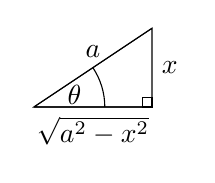
\begin{tikzpicture}[scale=0.5]
            \coordinate (A) at (-1.5cm,-1.0cm);
            \coordinate (B) at (1.5cm,1.0cm);
            \coordinate (C) at (1.5cm,-1.0cm);
            \draw (A) -- node[above]{\( a \)}
            (B) -- node[right]{\( x \)}
            (C) -- node[below]{\( \sqrt{a^2-x^2} \)}(A);
            \draw (C) -- (A) -- (B) pic [draw,angle radius=9mm,"\( \theta \)"]
                {angle=C--A--B};
            \draw (1.25cm,-1.0cm) rectangle (1.5cm,-0.75cm);
        \end{tikzpicture}
    \end{center}

    Tangent ($a^2+b^2x^2$, $x=\frac{a}{b}\tan{\left( \theta \right)}$)
    \begin{center}
        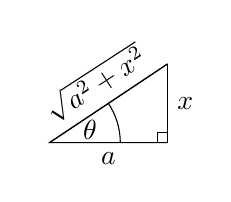
\begin{tikzpicture}[scale=0.5]
            \coordinate (A) at (-1.5cm,-1.0cm);
            \coordinate (B) at (1.5cm,1.0cm);
            \coordinate (C) at (1.5cm,-1.0cm);
            \draw (A) -- node [above, rotate=33] {\( \sqrt{a^2+x^2} \)} (B);
            \draw (B) -- node[right]{\( x \)} (C);
            \draw (C) -- node[below]{\( a \)}(A);
            \draw (C) -- (A) -- (B) pic [draw,angle radius=9mm,"\( \theta \)"]
                {angle=C--A--B};
            \draw (1.25cm,-1.0cm) rectangle (1.5cm,-0.75cm);
        \end{tikzpicture}
    \end{center}

    Secant ($b^2x^2-a^2$, $x=\frac{a}{b}\sec{\left( \theta \right)}$)
    \begin{center}
        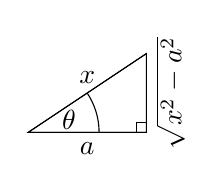
\begin{tikzpicture}[scale=0.5]
            \coordinate (A) at (-1.5cm,-1.0cm);
            \coordinate (B) at (1.5cm,1.0cm);
            \coordinate (C) at (1.5cm,-1.0cm);
            \draw (A) -- node[above]{\( x \)}
            (B) -- node[below, rotate=90]{\( \sqrt{x^2-a^2} \)}
            (C) -- node[below]{\( a \)}(A);
            \draw (C) -- (A) -- (B) pic [draw,angle radius=9mm,"\( \theta \)"]
                {angle=C--A--B};
            \draw (1.25cm,-1.0cm) rectangle (1.5cm,-0.75cm);
        \end{tikzpicture}
    \end{center}

    \section*{L'Hôpital's Rule}
    If $\displaystyle \lim_{x\to x_0}f(x)=\lim_{x\to x_0}g(x)=0$ or $\pm\infty$, then
    $\displaystyle \lim_{x\to x_0}\frac{f(x)}{g(x)} = \lim_{x\to x_0}\frac{f'(x)}{g'(x)}$.
    \section*{Continuity}
    $f(x)$ continuous at $c$ iff $\displaystyle \lim_{x\to c} f(x) = f(c)$.

    $f(x)$ is continuous on $I:\left( a,\:b \right)$ if it is continuous
    for all $x\in I$.

    $f(x)$ is continuous on $I:\left[ a,\:b \right]$ if it is continuous
    for all $x\in I$, but only right continuous at $a$ and left continuous at $b$.
    \section*{Intermediate Value Theorem}
    If $f(x)$ is continuous on $I:\left[ a, \: b \right]$ and $f(a) \leq c \leq f(b)$, then $\exists x\in I:f(x)=c$.
    \section*{Differentiability}
    $f(x)$ is differentiable at $x=x_0$ iff
    \begin{equation*}
        f'(x_0) = \lim_{x\to x_0} \frac{f(x)-f(x_0)}{x-x_0}
    \end{equation*}
    exists. This defines the derivative
    \begin{equation*}
        f'(x_0) = \lim_{h\to 0} \frac{f(x_0+h)-f(x_0)}{h}.
    \end{equation*}
    Differentiability implies continuity.
    \section*{Mean Value Theorem}
    If $f(x)$ is continuous and differentiable on $I:\left[ a,\:b \right]$, then
    \begin{equation*}
        \exists c\in I:f'(c)=\frac{f(b)-f(a)}{b-a}.
    \end{equation*}
    \section*{Definite Integrals}
    \begin{equation*}
        A = \int_a^b f(x) \dd{x}
    \end{equation*}
    \section*{Fundamental Theorem of Calculus}
    \begin{align*}
        \int_a^b \dv{x}F(x) \dd{x} & = F(b) - F(a) \\
        \dv{x}\int_a^x f(t) \dd{t} & = f(x)
    \end{align*}
    \section*{Taylor Polynomials / Series}
    \begin{equation*}
        f(x) \approx p_n(x) = \sum_{k=0}^n \frac{f^{\left( k \right)}(x_0)}{k!} \left( x-x_0 \right)^k
    \end{equation*}
    The Taylor Series is taking the limit as $n$ goes to infinity of $p_n$.

    \textbf{Maclaurin Series:} $x_0 = 0$.
    \section*{Common Maclaurin Series}
    \begin{table}[H]
        \centering
        \begin{tabular}{c | c | c}
            \toprule
            \textbf{Function}         & \textbf{Series Term}                                        & \textbf{Conv.}           \\
            \midrule
            $\e^{x}$                  & $\frac{x^n}{n!}$                                            & all $x$                  \\
            $\sin{\left( x \right)}$  & $\left( -1 \right)^n \frac{x^{2n+1}}{\left( 2n+1 \right)!}$ & all $x$                  \\
            $\cos{\left( x \right)}$  & $\left( -1 \right)^n \frac{x^{2n}}{\left( 2n \right)!}$     & all $x$                  \\
            $\frac{1}{1-x}$           & $x^n$                                                       & $\left( -1,\: 1 \right)$ \\
            $\frac{1}{1+x^2}$         & $\left( -1 \right)^n x^{2n}$                                & $\left( -1,\: 1 \right)$ \\
            $\ln{\left( 1+x \right)}$ & $\left( -1 \right)^{n+1} \frac{x^n}{n}$                     & $\left( -1,\: 1 \right]$ \\
            \bottomrule
        \end{tabular}
    \end{table}
    \textbf{Power Series:} $\sum_{n=0}^{\infty} c_n\left( x-x_0 \right)^n$
    \section*{Series Tests}
    For a series of the form $\displaystyle\sum_{i=i_0}^\infty a_i$:
    \section*{Alternating Series Test}
    Given $a_i = \left( -1 \right)^i b_i$ and $b_i>0$.

    If $b_{i+1}\leqslant b_i$ \& $\lim_{i\to\infty}b_i=0$, then
    convergent, else inconclusive.
    \section*{Ratio Test}
    Given $\rho = \lim_{i\to\infty}\abs{\frac{a_{i+1}}{a_i}}$:
    \begin{align*}
        \rho < 1 & : \text{convergent}   \\
        \rho > 1 & : \text{divergent}    \\
        \rho = 1 & : \text{inconclusive}
    \end{align*}
    \section*{Multivariable Functions}
    \textbf{Partial Derivatives} are done w.r.t one variable, other variables unchanged.

    The \textbf{Gradient} is $\symbf{\nabla}f = \avec[\big]{\pdv{f}{x},\: \pdv{f}{y},\: \dots}$
    \section*{Level Curves}
    \begin{equation*}
        L_c\left( f \right) = \bigl\{ \left( x,\: y \right) : f\left(x,\: y\right) = c\bigr\}
    \end{equation*}
    If $f(x,\: y) \to L$ as $(x,\: y) \to (x_0,\: y_0)$, then
    $\displaystyle \lim_{(x,\: y) \to (x_0,\: y_0)} = L$ along any smooth
    curve. The limit does not exist if $L$ changes along different smooth curves.

    \section*{Multivariable Chain Rule}
    For $\pdv{f}{s}$, create a tree from $f$ to the variable $s$.
    On each edge, where the node above is $a$ and below is $b$, each edge is $\pdv{a}{b}$.
    Traverse each path between $f$ and $s$ and multiply the edges.
    Add each path together.
    (i.e. for $f(x, y), x(s,t), y(s,t)$, $\pdv{f}{s} = \pdv{f}{x}\pdv{x}{s}+\pdv{f}{y}\pdv{y}{s}$)
    \section*{Directional Derivatives}
    \begin{align*}
        \symbf{D}_{\symbfit{u}}f = \symbf{\nabla}_{\symbfit{u}}f
         & = \symbf{\nabla}f \cdot \symbfit{u}
    \end{align*}
    where $\symbfit{u}$ is a unit vector and the slope is given by $\norm{\symbf{\nabla}_{\symbfit{u}}f}$.
    If $\symbf{\nabla}_{\symbfit{u}}f=0$, $\symbfit{u}$ is tangent to the level curve at $\symbfit{x}_0$.
    \begin{align*}
        \max_{\norm{\symbfit{u}} = 1} \symbf{\nabla}_{\symbfit{u}}f = \symbf{\nabla}f
    \end{align*}
    If $\symbf{\nabla}f\neq 0$, $\symbf{\nabla}f$ is a normal vector to the level curve at $\symbfit{x}_0$.
    \section*{Critical Points}
    $(x_0,\: y_0)$ is a critical point if $\symbf{\nabla}f(x_0,\: y_0) = \symbf{0}$
    or if $\symbf{\nabla}f(x_0,\: y_0)$ is undefined.
    \section*{Classification of Critical Points}
    \begin{equation*}
        D = f_{xx}f_{yy} - \left( f_{xy} \right)^2
    \end{equation*}
    \begin{description}
        \item[$D > 0$ and $f_{xx} < 0$:] local maxima
        \item[$D > 0$ and $f_{xx} > 0$:] local minima
        \item[$D < 0$:] saddle point
        \item[$D = 0$:] inconclusive
    \end{description}
    \section*{Double Integrals}
    The volume of the solid
    enclosed between the surface $z=f(x,\: y)$ and the region $\Omega$ is
    defined by
    \begin{equation*}
        V = \iint\limits_{\Omega} f(x,\: y) \dd{A}.
    \end{equation*}
    If $\Omega$ is a region bounded by $a \leq x \leq b$ and $c \leq y \leq d$, then
    \begin{align*}
        \iint\limits_{\Omega} f(x,\: y) \dd{A} & = \int_c^d\int_a^b f(x,\: y) \dd{x} \dd{y} \\
                                               & = \int_a^b\int_c^d f(x,\: y) \dd{y} \dd{x}
    \end{align*}
    \section*{Type I Regions}
    \begin{equation*}
        \iint\limits_{\Omega} f(x,\: y) \dd{A} = \int_a^b\int_{g_1(x)}^{g_2(x)} f(x,\: y) \dd{y} \dd{x}
    \end{equation*}
    \textbf{Bounded left \& right by:}
    \begin{equation*}
        x=a \text{ and } x=b
    \end{equation*}
    \textbf{Bounded below \& above by:}
    \begin{equation*}
        y=g_1(x) \text{ and } y=g_2(x)
    \end{equation*}
    where $g_1(x) \leq g_2(x)$ for $a \leq x \leq b$:
    \section*{Type II Regions}
    \begin{equation*}
        \iint\limits_{\Omega} f(x,\: y) \dd{A} = \int_c^d\int_{h_1(x)}^{h_2(x)} f(x,\: y) \dd{x} \dd{y}
    \end{equation*}
    \textbf{Bounded left \& right by:}
    \begin{equation*}
        x=h_1(y) \text{ and } x=h_2(y)
    \end{equation*}
    \textbf{Bounded below \& above by:}
    \begin{equation*}
        y=c \text{ and } y=d
    \end{equation*}
    where $h_1(y) \leq h_2(y)$ for $c \leq y \leq d$.

    To integrate, solve the inner integrals first.
    \section*{Vector Valued Functions}
    \begin{equation*}
        \symbf{r}:\mathbb{R} \to \mathbb{R}^n
    \end{equation*}
    The \textbf{domain} of $\symbf{r}(t)$ is the intersection of the domains
    of its components.

    The \textbf{orientation} of $\symbf{r}(t)$ is the direction of motion along the
    curve as the value of the parameter increases.

    \textbf{Limits}, \textbf{derivatives} and \textbf{integrals} are all \textit{component-wise}. Each component has its \underline{own} constant of integration.
    \section*{Parametric Lines}
    \begin{equation*}
        \symbf{l}(t) = \symbfit{P}_0 + t\symbfit{v}
    \end{equation*}
    where $\symbf{l}(t)$ passes through $\symbfit{P}_0$, and is parallel to $\symbfit{v}$.
    \section*{Tangent Lines}
    If $\symbf{r}(t)$ is differentiable at
    $t_0$ and $\symbf{r'}(t_0)\ne\symbf{0}$
    \begin{equation*}
        \symbf{l}(t) = \symbf{r}(t_0)+t\symbf{r'}(t_0).
    \end{equation*}
    \section*{Curves of Intersection}
    Choose one of the variables as the parameter, and express the remaining variables in terms of that parameter.
    \section*{Arc Length}
    \begin{equation*}
        S = \int_a^b \norm{\symbf{r'}(t)} \dd{t}
    \end{equation*}
    \section*{Ordinary Differential Equations}
    \textbf{Order:} highest derivative in DE.

    \textbf{Autonomous DE:} does not depend explicitly on the independent variable.
    \section*{Qualitative Analysis}
    \begin{equation*}
        \dv{y}{t} = f(y)
    \end{equation*}
    A fixed point is the value of $y$ for which $f(y) = 0$.
    \section*{Stability of Fixed Points}
    Given a positive/negative perturbation from a fixed point, that point is

    \textbf{Stable:} if both tend toward FP

    \textbf{Unstable:} if both tend away from FP

    \textbf{Semi-Stable:} if one tends toward FP, and another tends away from FP
    \section*{Directly Integrable ODEs}
    For $\dv{y}{x} = f(x)$:
    \begin{equation*}
        y(x) = \int f(x) \dd{x}.
    \end{equation*}
    \section*{Separable ODEs}
    For $\dv{y}{x} = p(x) q(y)$:
    \begin{equation*}
        \int \frac{1}{q(y)} \dv{y}{x} \dd{x} = \int p(x) \dd{x}.
    \end{equation*}
    \section*{Linear ODEs}
    For $\dv{y}{x} + p(x)y = q(x)$, use the \textit{integrating factor}:
    $I(x) = \e^{\int p(x) \dd{x}}$, so that
    \begin{equation*}
        y(x) = \frac{1}{I(x)} \int I(x) q(x) \dd{x}.
    \end{equation*}
    \section*{Exact ODEs}
    $P(x,\: y) + Q(x,\: y)\dv{y}{x} = 0$
    has the solution
    $\Psi(x,\: y) = c$
    iff it is exact, namely, when
    $P_y = Q_x$,
    where $P = \Psi_x$ and $Q = \Psi_y$. Then
    \begin{gather*}
        \Psi(x,\: y) = \int P(x,\: y) \dd{x} + f(y) \\
        \Psi(x,\: y) = \int Q(x,\: y) \dd{y} + g(x)
    \end{gather*}
    and $f(y)$ and $g(x)$ can be determined by solving these equations simultaneously.
    \section*{Second-Order ODEs}
    \begin{equation*}
        a_2(x)y'' + a_1(x)y' + a_0(x)y = F(x)
    \end{equation*}
    \section*{Initial Values}
    \begin{align*}
        y(x_0) = y_0 \quad y'(x_0) = y_1
    \end{align*}
    \section*{Boundary Values}
    \begin{align*}
        y(x_0) = y_0 \quad y(x_1) = y_1
    \end{align*}
    \section*{Reduction of Order}
    \begin{equation*}
        y_2(x) = v\left(x\right) y_1(x)
    \end{equation*}
    $v(x)$ can be determined by substituting $y_2$ into the ODE, using $w(x) = v'(x)$.
    \section*{General Solution}
    \begin{equation*}
        y(x) = y_H(x) + y_P(x)
    \end{equation*}
    \section*{Homogeneous Solution}
    \begin{equation*}
        y_H(x) = \e^{\lambda x}
    \end{equation*}
    \section*{Real Distinct Roots}
    \begin{equation*}
        y_H(x) = c_1\e^{\lambda_1 x} + c_2\e^{\lambda_2 x}
    \end{equation*}
    \section*{Real Repeated Roots}
    \begin{equation*}
        y_H(x) = c_1\e^{\lambda x} + c_2 t\e^{\lambda x}
    \end{equation*}
    \section*{Complex Conjugate Roots}
    Given $\lambda = \alpha \pm \beta i$:
    \begin{equation*}
        y_H(x) = \e^{\alpha x}\bigl( c_1\cos{\left( \beta x \right)} + c_2 \sin{\left( \beta x \right)} \bigr)
    \end{equation*}
    \section*{Particular Solution}
    \begin{table}[H]
        \centering
        \begin{tabular}{c | c}
            \toprule
            $F(x)$                                                             & $y_P(x)$                               \\
            \midrule
            constant                                                           & A                                      \\
            polynomial degree $n$                                              & $\displaystyle \sum_{i = 0}^n A_i x^i$ \\
            $\e^{kx}$                                                          & $A \e^{kx}$                            \\
            $\cos{\left( \omega x \right)}$ or $\sin{\left( \omega x \right)}$ & $A_0 \cos{\left( \omega x \right)}$    \\ & $+ A_1 \sin{\left( \omega x \right)}$ \\
            \bottomrule
        \end{tabular}
    \end{table}
    If $F(x)$ is a combination of the above, $y_P(x)$ should be too.
    If the choice would be linearly dependent to $y_H(x)$, multiply by $x$ until it isn't.

    Substitute $y_P$ into the nonhomogeneous ODE, and solve the undetermined coefficients.
    \section*{Spring and Mass Systems}
    \begin{equation*}
        m y'' + \gamma y' + k y = f(t)
    \end{equation*}
    \textbf{Newton's Law:} $F = m y''$

    \textbf{Spring force:} $F_s = -k y$

    \textbf{Damping force:} $F_d = -\gamma y'$
    \begin{align*}
        m      & : \text{mass}    & k    & : \text{spring constant} \\
        \gamma & : \text{damping} & f(t) & : \text{external force}
    \end{align*}
    \section*{Electrical Circuits}
    The sum of voltages around a loop equals 0.
    \begin{align*}
        v(t) - iR - L \dv{i}{t} - \frac{q}{C}      & = 0    \\
        L \dv[2]{q}{t} + R\dv{q}{t} + \frac{1}{C}q & = v(t)
    \end{align*}
    where $\displaystyle i = \dv{q}{t}$.
    \begin{align*}
        R & : \text{resistance} & C    & : \text{capacitance}    \\
        L & : \text{inductance} & v(t) & : \text{voltage supply}
    \end{align*}

\end{multicols}
\end{document}
